Motstand og ledningsevne påvirkes av temperaturforandring.
\\\\
Ledere:\\
Motstanden i en leder har en positiv temperaturkoeffisient
og \emph{øker} med temperaturen.
Det er fordi elektronene kolliderer med hverandre.
\\\\
Halvledere:\\
Motstanden har negativ temperaturkoeffisient
og motstanden synker fordi
elektroner blir termisk eksitert opp til ledningsbåndet.
\\
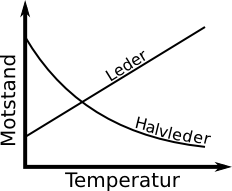
\includegraphics[width=0.5\textwidth]{./img/temperatur}
